\chapter{Implementation: InvestiGator}
\label{cap:sistema}

This chapter describes the realisation of the system: its architecture, the way each method of
Chapter~\ref{cap:metodologia} is put into effect, the policy that decides what is communicated to
the user, the construction of the message delivered, and the life cycle of the learned
component.

Chapter~\ref{cap:metodologia} presented four methods in isolation. Composing them into a working
system introduces problems that none of them presents on its own: the unavailability of the
sources, the volume of candidates per cycle, the coherence between the values computed and the text
presented, and the silent degradation of the components over time. The description that follows is
organised around those problems.

The system developed is called InvestiGator and is in continuous operation, delivering alerts to a
messaging channel and making the record of its decisions available in a web application. The values
presented in this chapter were read from the log of the system in operation, and the dates on which
each measurement was taken are indicated alongside each one.

\section{System architecture}
\label{sec:sis_arquitetura}

The architecture of InvestiGator was defined according to the following requirements, concerning
cost, modularity, verifiability and resilience:

\begin{itemize}
  \item to operate exclusively on free data sources, with no subscriptions and no per-request
        costs;
  \item to isolate each method in a component with a single responsibility, replaceable without
        changing the others;
  \item to guarantee that any value presented to the user originates in the component that
        computed it, and not in a second independent derivation;
  \item to tolerate the unavailability of any external source without interrupting the service;
  \item to record every decision taken, including the decisions not to communicate.
\end{itemize}

The system is organised into five components, shown in Figure~\ref{fig:sis_arquitetura}:
detection, retrieval, triage, explanation and delivery. The decomposition of the movement is a
sixth component, activated only on the path started by a price movement, since the split applies to
the return of the day and there is no object to split when the event that triggers the assessment
is a news item.

\begin{figure}[ht]
\centering
\begin{tikzpicture}[
  font=\small, >={Stealth[length=2.4mm]},
  cx/.style={draw, rounded corners, align=center, text width=2.6cm, minimum height=1.5cm,
             inner sep=4pt},
  fonte/.style={cx, fill=black!10},
  proc/.style={cx, fill=black!3},
  saida/.style={cx, fill=black!16},
]
  \node[fonte] (p) {\textbf{Prices}\\ \footnotesize chain of five\\ \footnotesize sources};
  \node[fonte, below=6mm of p] (n) {\textbf{News}\\ \footnotesize three free\\ \footnotesize interfaces};
  \node[fonte, below=6mm of n] (h) {\textbf{Case base}\\ \footnotesize precedents with\\ \footnotesize measured impact};

  \node[proc, right=0.8cm of p] (det) {\textbf{Detection}\\ \footnotesize $z$-score};
  \node[proc, right=0.8cm of n] (rec) {\textbf{Retrieval}\\ \footnotesize semantic neighbours};
  \node[proc, right=0.8cm of h] (tri) {\textbf{Triage}\\ \footnotesize calibrated probability};
  \node[proc, dashed, below=6mm of tri] (dec)
    {\textbf{Decomposition}\\ \footnotesize market, sector,\\ \footnotesize company};

  \node[proc, right=0.9cm of rec, text width=2.8cm] (exp)
    {\textbf{Explanation}\\ \footnotesize composed from\\ \footnotesize the computed\\ \footnotesize objects};

  \node[saida, right=0.8cm of exp, yshift=9mm] (tg) {\textbf{Messaging channel}};
  \node[saida, right=0.8cm of exp, yshift=-9mm] (web) {\textbf{Web application}\\ \footnotesize decision log};

  \draw[->] (p) -- (det);
  \draw[->] (n) -- (rec);
  \draw[->] (h) -- (tri);
  \draw[->] (h.east) -- ++(0.35,0) |- (rec.west);
  \draw[->] (det.east) -- ++(0.4,0) |- (exp.west);
  \draw[->] (rec) -- (exp);
  \draw[->] (tri.east) -- ++(0.4,0) |- (exp.west);
  \draw[->, dashed] (p.south west) -- ++(-0.35,0) |- (dec.west);
  \draw[->, dashed] (dec.east) -- ++(0.55,0) |- (exp.west);
  \draw[->] (exp.east) -- ++(0.35,0) |- (tg.west);
  \draw[->] (exp.east) -- ++(0.35,0) |- (web.west);
\end{tikzpicture}
\caption[Architecture of InvestiGator]{Components of the system and their connections. On the
left, the data sources; in the centre, the methods of Chapter~\ref{cap:metodologia} and the
component that composes the text; on the right, the two delivery channels. The decomposition is
dashed because it is the only component that does not take part in every assessment.}
\label{fig:sis_arquitetura}
\end{figure}

One construction rule runs through the whole implementation: the text delivered to the user is
composed from the objects the components produced, and not written independently. When the detector
computes a $z$ value equal to $+7.61$, it is that value the message presents. The alternative,
which would consist in keeping one place where the text is written and another where the quantity
is computed, admits divergence between the two without that divergence being observable. The
constraint eliminates that possibility by construction.

\subsection{Communication between components}

The components communicate by direct passing of objects within a single process, and not by
network protocol. The decision follows from the usage profile: the system serves a small list of
companies, with a sixty-second assessment cycle, and the volume does not justify the coordination
cost of a distributed architecture. The separation between components is ensured by explicit
interfaces, which preserves replaceability without introducing communication latency.

Two exceptions operate across process boundaries. Delivery uses the bot interface of the messaging
channel, by \gls{HTTP} request. The web application that exposes the decision log runs as a
separate process and reads the same data store, without writing to it. This second separation
guarantees that consulting the log does not interfere with the assessment cycle.

\section{Data acquisition}
\label{sec:sis_dados}

The zero-cost constraint determines the acquisition decisions. A retail investor who considers
brokerage costs high does not subscribe to a financial information terminal, and the usefulness of
the system for the recipient defined in Chapter~\ref{cap:introducao} depends on the system
operating without that cost. Free sources present, however, three systematic limitations: they
block access for excess of requests, they answer with an error without warning, and they publish
late. The decisions described in this section respond to those limitations.

\subsection{Quotes}

Prices are obtained through a chain of five sources, consulted in a fixed order, the first that
answers with valid data being adopted. The identifier of the source that served each value is
recorded together with the value, since the provenance of a quantity is part of its
explanation.

The order of the chain is neither arbitrary nor definitive. One of the sources was demoted after
it began answering with an anti-robot check, which makes it unusable in a reliable way in
automated operation; it remains in the chain, in a lower position, as an opportunistic attempt.
The decision resulted from observing what the source returned, and not from declared preference.

The redundancy of the chain has a consequence that goes beyond availability. Without it, a day on
which the single source blocks access is indistinguishable from a day on which the market did not
open, and the system has no way of separating the two situations.

\subsection{News}
\label{sec:sis_fontes}

News is obtained per company, from three free interfaces. The material received includes a high
volume of unusable content: automatic lists of the day's largest movers, texts that mention the
company only in passing, and press releases from law firms. A relevance filter, applied on entry,
requires the headline to name the company explicitly and rejects the known patterns of
automatically generated text.

The use of three sources rather than one was assessed by measurement, over twelve companies and
three days. The criterion adopted is not the number of headlines returned by each source, but the
number of headlines that survives the relevance filter, since material rejected on entry never
comes to exist for the system. Table~\ref{tab:sis_fontes} presents the result.

\begin{table}[!htbp]
\caption[Characterisation of the three news sources]{Material delivered by each free source after
the relevance filter is applied. The \emph{exclusive} column indicates the headlines that one
source brings and none of the others brings. That value is an upper bound, since the comparison
between headlines is made by textual matching after normalisation, and two sources that describe
the same event in different words produce two headlines counted as distinct.}
\label{tab:sis_fontes}
\centering
\small
\begin{tabular}{L{0.20\textwidth} C{0.12\textwidth} C{0.11\textwidth} C{0.13\textwidth}
                C{0.12\textwidth} C{0.13\textwidth}}
\toprule
\tabhead{Source} & \tabhead{Relevant} & \tabhead{Precision} & \tabhead{Freshness} &
\tabhead{Coverage} & \tabhead{Exclusive} \\
\midrule
Finnhub & $432$ & $\mathbf{35\%}$ & $15.8$ h & $\mathbf{12/12}$ & $401$ \\
Alpha Vantage & $141$ & $24\%$ & $\mathbf{9.3}$ \textbf{h} & $\mathbf{12/12}$ & $119$ \\
Polygon & $429$ & $27\%$ & $52.6$ h & $8/12$ & $\mathbf{418}$ \\
\bottomrule
\end{tabular}
\end{table}

The three sources have complementary profiles, and it is that complementarity, and not the
aggregate volume, that justifies using them together. Finnhub has the highest labelling precision
and covers all the companies. Alpha Vantage has the lowest median age of the news, at $9.3$ hours
against $15.8$, which makes it the relevant source for reducing the delay of the alerts. Polygon
contributes the largest number of exclusive headlines, with a median age of $52.6$ hours, which
makes it suitable for feeding the case base and unsuitable for alerting in useful time. That is the
use assigned to it.

The three sources together produce $970$ distinct relevant headlines, against the $432$ obtained
with Finnhub alone. The gain concentrates on the companies with the lowest individual coverage,
which are precisely the cases in which the system previously had no material to comment on.

Aggregation does not, however, guarantee a reduction in latency in general. The three sources
publish with delays of their own, and the gain in a concrete case depends on which of them observed
the event first. The median freshness improves, and that improvement is measured; the claim that
alerts now arrive earlier would require a new end-to-end latency measurement over an extended
period, which was not carried out.

\subsection{Historical base and deployed base}

Precedent retrieval requires a body of past cases with a known outcome. The system uses two
distinct sets, with distinct purposes, and their separation matters for reading the results of
Chapter~\ref{cap:avaliacao}.

The first is \gls{FNSPID} \autocite{dong2024fnspid}, a public set of financial news aligned with
the corresponding prices. From the alignment described in Section~\ref{sec:met_dados} result
$79{,}753$ examples between 2018 and 2023, each with the subsequent price movement. It is on this
set that the methods are evaluated.

The second is the case base the deployed system consults, and it results from merging two origins
that should not be confused. The first is a reconstruction of one year of history, obtained by
running the collection and maturation components over the past, with $38{,}214$ cases; the
separation from the log of the running system is deliberate, since a replayed case is not an
observed case. The second is the live base, fed by the scan, with $11{,}445$ cases as of 20 August 2026, and
growing with operation. Retrieval scans
both together. The vectors are stored as a single-precision matrix mapped on disk. The format is
not indifferent: the same representations in the language's native structures exceeded the memory
available in the execution container, and the change of format was the condition that made their
use possible.

\section{The path of an event}
\label{sec:sis_percurso}

The system admits two distinct paths, depending on whether the event that triggers the assessment
is a news item or a price movement. The two converge in the explanation component and use the same
decision policy, described in Section~\ref{sec:sis_politica}.

\subsection{Path started by a news item}

The path started by a news item comprises nine stages, shown in
Figure~\ref{fig:sis_caminho}. Five of those stages are decision points at which the candidate can
be discarded, in which case the system does not communicate.

\begin{figure}[ht]
\centering
\begin{tikzpicture}[
  font=\footnotesize, >={Stealth[length=2mm]},
  et/.style={draw, rounded corners, align=center, text width=2.15cm, minimum height=1.15cm,
             fill=black!3},
  porta/.style={et, dashed, fill=black!12},
  n/.style={font=\bfseries\footnotesize, text=black!45},
]
  \node[et] (a) {collect\\ news};
  \node[porta, right=4mm of a] (b) {names the\\ company?};
  \node[porta, right=4mm of b] (c) {is it recent?};
  \node[et, right=4mm of c] (d) {retrieve\\ precedents};
  \node[porta, below=7mm of d] (e) {enough\\ evidence?};
  \node[porta, left=4mm of e] (f) {triage\\ above the\\ floor?};
  \node[porta, left=4mm of f] (g) {already sent\\ today?};
  \node[et, left=4mm of g] (h) {compose the\\ explanation};
  \node[et, below=7mm of h, fill=black!16] (i) {deliver and\\ log};

  \foreach \x/\i in {a/1, b/2, c/3, d/4} { \node[n, above=0.5mm of \x] {\i}; }
  \foreach \x/\i in {f/6, g/7, h/8} { \node[n, above=0.5mm of \x] {\i}; }
  % Estas duas caixas recebem a seta pelo TOPO: um numero centrado ficaria por baixo
  % dela, riscado, que e' como estiveram ate 2026-09-05. Deslocados para o lado.
  \node[n] at ([xshift=6mm,yshift=2.6mm]e.north west) {5};
  \node[n] at ([xshift=6mm,yshift=2.6mm]i.north west) {9};

  \draw[->] (a) -- (b); \draw[->] (b) -- (c); \draw[->] (c) -- (d);
  \draw[->] (d) -- (e); \draw[->] (e) -- (f); \draw[->] (f) -- (g); \draw[->] (g) -- (h);
  \draw[->] (h) -- (i);
\end{tikzpicture}
\caption[Stages of the path started by a news item]{The nine stages of the path. The dashed boxes
correspond to decision points at which the candidate can be discarded.
Section~\ref{sec:sis_politica} quantifies the proportion of candidates eliminated at each one.}
\label{fig:sis_caminho}
\end{figure}

The operation of the path is illustrated by an alert delivered on 12 July 2026, concerning Meta,
with the headline \emph{``Mark Zuckerberg Said Meta's AI Bets `Haven't Come to Fruition Yet' as
Shares Fell 5\%''}. The headline names the company and matches none of the automatic text patterns.
The date falls within the two-day interval required. The three closest precedents are Microsoft of
2023-11-07, with similarity $0.46$, Nvidia of 2023-08-02, with $0.51$, and Nvidia of 2023-09-21,
with $0.46$; the best of them is above the $0.45$ threshold. The triage model assigns a probability
of $54\%$. And the alert is the first concerning the company on that day. The message is then
composed and logged.

The precedents retrieved in this case belong to companies distinct from the one the alert concerns,
and are presented nonetheless. The option is deliberate and follows from the formulation of the
second research question: comparability is established by the topic of the news and not by the
identity of the company. News items concerning investment in artificial intelligence at large
technology companies are cases comparable with one another.

The outcomes of the three precedents diverge, with movements of $+2.70\%$, $-3.87\%$ and
$+5.05\%$. The system presents the three individually, and not their average, precisely for that
reason. The average hides the most relevant piece of information in the set, which is the absence
of a common outcome across similar cases.

\subsection{Path started by a price movement}

The second path is substantially shorter. The $z$-score is computed by two routes. After the close
of each session, the system assesses the return of the closed day of each company on the watched
list against the norm of the twenty preceding days, as described in Section~\ref{sec:met_detecao}.
During the session, it assesses the return in progress, obtained from the current quote against the
previous close, against the same daily norm, formed in that case by the twenty most recent complete
days, since the day in progress does not yet belong to the series. The second route brings the
detection forward without changing the definition of normality, and is what allows a movement to be
communicated while the session is under way; it is also the one that does not depend on the
historical series source, whose bar for the day may arrive late. On either route, crossing the
threshold is a sufficient condition for assessment.

It is on this path, and only on this one, that the decomposition of the movement intervenes. A line
is added to the alert with the split computed according to Section~\ref{sec:met_decomposicao}, in
the form \emph{``NFLX $-2.11\%$ today $=$ $-0.08\%$ market $\cdot$ $-0.32\%$ sector $\cdot$
$-1.71\%$ company itself''}, followed by a sentence that names in plain language the dominant part.
When estimating the sensitivity to the market is not possible, the line is presented all the same,
declaring that unit sensitivity was assumed and that the split is indicative.

Two capabilities were added to the path after the system entered operation, both from observing its
behaviour in production. The first consists in assigning severity levels: a $z$ value of $1.6$ and a
value of $3.2$ came to be described by distinct terms, instead of producing the same wording. The
second consists in comparing with the remaining companies of the same sector in the same session,
since an alert that reports a fall without indicating that the whole sector fell conveys incomplete
information.

The second correction resulted from reading the first thirty alerts delivered. In nine of them the
text was internally contradictory: one line indicated that the movement appeared to be common to
the sector, and the split presented two lines below attributed the largest part to the company. The
two lines were correct in isolation, and the contradiction resulted from the comparison with peers
considering only the direction of the movement of the neighbouring companies, and not its
magnitude. The comparison came to consider both.

\section{Decision policy}
\label{sec:sis_politica}

Communicating every candidate assessed is equivalent to communicating nothing. A channel that
delivers fifteen messages a day stops being read, and the system loses the usefulness that
justifies its existence. The decision points of Figure~\ref{fig:sis_caminho} respond to this
constraint.

\subsection{Observed selectivity}

The joint effect of the decision points is considerable. Over the news dated between 1 and 3
September 2026, the system assessed $743$ distinct headlines from twelve companies and delivered
$15$ alerts, which corresponds to a ratio of roughly one in fifty. The window is short, and the
decision log that supports it keeps three days, which fixes its limit.
Figure~\ref{fig:sis_seletividade} presents the distribution by company.

The budget is, in the configuration in operation, the constraint that actually binds. Over the
production decision log, and on each of the six days measured, between $77.7\%$ and $99.8\%$ of the
assessments end there, against a maximum of $4.6\%$ at the similarity threshold and of $14.0\%$ at
the same-day repetition check. The reading is not that the remaining gates are useless: it is that
the reduction in volume that matters has already occurred before them, in the relevance filter and
in the selection of one headline per company per cycle, and that from there on the governed
quantity is the daily total. It is also the direct consequence of the policy change described in
Section~\ref{sec:av_producao}: the model ceased to exercise a veto and came to rank within the
budget, so the budget being the active constraint is the policy behaving as it was designed, and
not a departure from it.

Two clarifications condition the reading of these numbers, and the second is the more important.
The first is that the unit is the distinct headline: the system re-assesses the same headlines at
every cycle, so the log contains $1{,}321$ rows for the $743$ headlines, and counting assessments
would inflate the funnel. The second is that the total of fifteen alerts does not measure the raw
material available, but the policy: the daily budget of five was used in full on all three days, so
fifteen is the ceiling the policy imposes and not an observed quantity. What the distribution by
company measures is the ordering within that ceiling, and that is not imposed: no company has a
quota of its own.

\begin{figure}[ht]
\centering
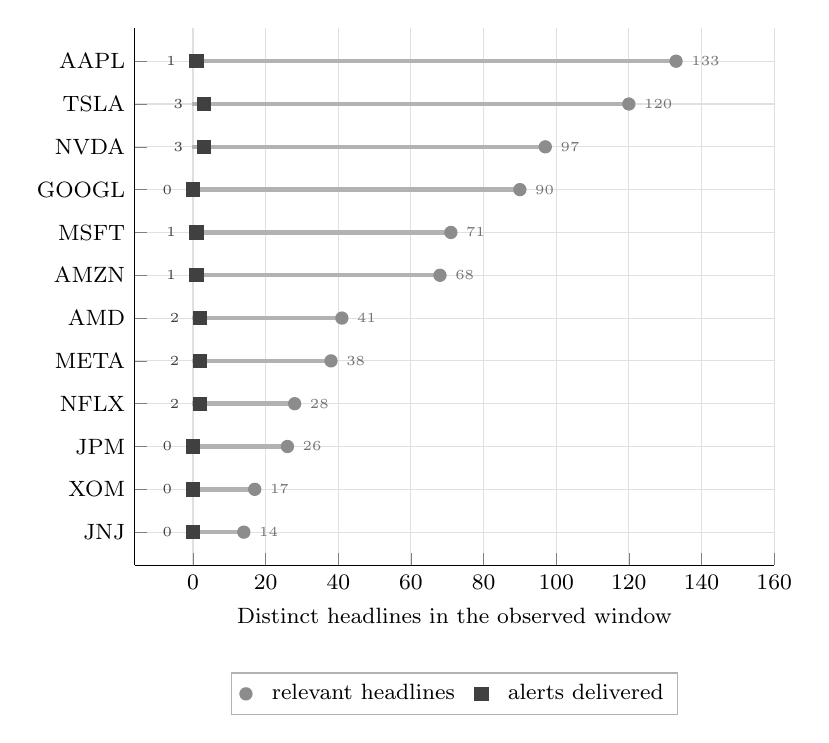
\begin{tikzpicture}
\begin{axis}[
  % Lollipop, e nao barras emparelhadas: quatro das doze empresas tem zero alertas, e num
  % grafico de barras o zero e' uma barra invisivel -- comunicava-se por ausencia. O marcador
  % quadrado esta sempre presente, e onde vale zero esta rotulado.
  % DADOS: docs/evaluation/evaluation_funil_seletividade.md, janela 2026-09-01 a 2026-09-03.
  % O instantaneo anterior (2026-07-13) foi retirado por quatro defeitos diagnosticados a
  % 2026-09-04: comparava uma janela deslizante com um cumulativo, o rotulo da janela nao era
  % a janela contada, o valor 14 repetido em tres empresas era o TECTO de 2/empresa/dia, e a
  % politica que descrevia foi substituida a 2026-08-15 pelo orcamento global.
  width=0.80\textwidth, height=8.4cm,
  % ⚠ A margem esquerda existe para a contagem de alertas caber entre
  % o eixo e o marcador do zero. Com -6 os zeros saiam por cima da linha do
  % eixo e liam-se como noves, nas empresas cuja leitura mais interessa.
  xmin=-16, xmax=160,
  enlarge y limits=0.07,
  symbolic y coords={JNJ,XOM,JPM,NFLX,META,AMD,AMZN,MSFT,GOOGL,NVDA,TSLA,AAPL},
  ytick={JNJ,XOM,JPM,NFLX,META,AMD,AMZN,MSFT,GOOGL,NVDA,TSLA,AAPL},
  xlabel={Distinct headlines in the observed window},
  tick label style={font=\footnotesize},
  label style={font=\footnotesize},
  legend style={font=\footnotesize, at={(0.5,-0.20)}, anchor=north, legend columns=2,
                draw=black!30, column sep=1.2ex},
  grid=major, grid style={black!12},
  axis lines*=left,
  ]
  % haste: do zero ate ao numero de titulos
  \addplot[xbar, bar width=1.2pt, fill=black!30, draw=black!30, forget plot]
    coordinates {(14,JNJ) (17,XOM) (26,JPM) (28,NFLX) (38,META) (41,AMD) (68,AMZN) (71,MSFT) (90,GOOGL) (97,NVDA) (120,TSLA) (133,AAPL)};
  \addplot[only marks, mark=*, mark size=2.2pt, black!45,
           nodes near coords, point meta=explicit symbolic,
           every node near coord/.append style={font=\tiny, black!55, anchor=west, xshift=2pt}]
    coordinates {(14,JNJ) [14] (17,XOM) [17] (26,JPM) [26] (28,NFLX) [28] (38,META) [38] (41,AMD) [41] (68,AMZN) [68] (71,MSFT) [71] (90,GOOGL) [90] (97,NVDA) [97] (120,TSLA) [120] (133,AAPL) [133]};
  \addplot[only marks, mark=square*, mark size=2.4pt, black!75,
           nodes near coords, point meta=explicit symbolic,
           % ⚠ ABAIXO do marcador, e nao a esquerda: os zeros ficavam em cima da linha
           % do eixo e liam-se como noves, o que invertia a leitura das empresas que
           % nao alertam.
           every node near coord/.append style={font=\tiny, black!75,
                                                anchor=east, xshift=-4pt}]
    coordinates {(0,JNJ) [0] (0,XOM) [0] (0,JPM) [0] (2,NFLX) [2] (2,META) [2] (2,AMD) [2] (1,AMZN) [1] (1,MSFT) [1] (0,GOOGL) [0] (3,NVDA) [3] (3,TSLA) [3] (1,AAPL) [1]};
  \legend{relevant headlines, alerts delivered}
\end{axis}
\end{tikzpicture}
\caption[Selectivity of the system by company]{Distinct headlines assessed and alerts actually
delivered, by company, between 1 and 3 September 2026. The total is $743$ headlines and $15$
alerts, and the two quantities are counted over the same window. The total of alerts is the ceiling
the daily budget imposes, and not a measurement; what the figure shows is the distribution of that
ceiling, which the policy does not fix. Eight of the twelve companies receive at least one alert,
and the company with the most headlines assessed is not the most alerted.
Section~\ref{sec:av_producao} examines the effect of this policy over a much larger window.}
\label{fig:sis_seletividade}
\end{figure}


The behaviour on a single day makes it possible to locate where candidates are eliminated.
Figure~\ref{fig:sis_funil} distributes the $5{,}060$ assessments recorded on 15 August 2026 by the
decision point at which each one ended. The log read corresponds to part of the day and not to the
complete day, so the values should be read as proportions.

\begin{figure}[ht]
\centering
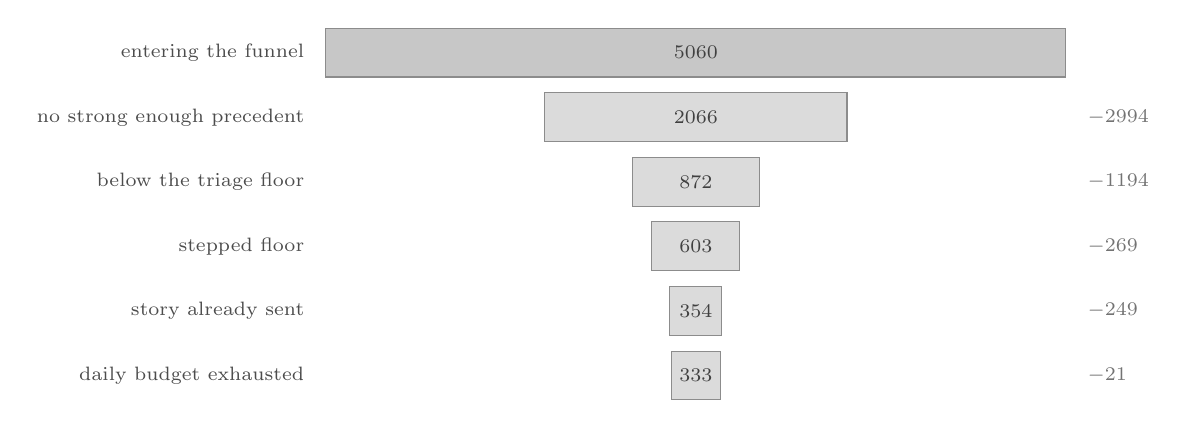
\begin{tikzpicture}[font=\footnotesize]
  % Funil a serio: a largura e' o QUE RESTA depois de cada porta, e o rotulo a direita e' o que
  % essa porta cortou. A forma de barras dava os cortes e escondia o resto acumulado, que e' a
  % leitura que interessa: 5060 menos 2994, 1194, 269, 249 e 21 da exactamente 333.
  \fill[black!22, draw=black!45] (-4.70,0.00) rectangle (4.70,-0.62);
  \node[font=\scriptsize, black!75] at (0,-0.31) {5060};
  \node[left, font=\scriptsize, black!70, align=right] at (-4.85,-0.31) {entering the funnel};
  \fill[black!14, draw=black!45] (-1.92,-0.82) rectangle (1.92,-1.44);
  \node[font=\scriptsize, black!75] at (0,-1.13) {2066};
  \node[left, font=\scriptsize, black!70, align=right] at (-4.85,-1.13) {no strong enough precedent};
  \node[right, font=\scriptsize, black!55] at (4.85,-1.13) {$-$2994};
  \fill[black!14, draw=black!45] (-0.81,-1.64) rectangle (0.81,-2.26);
  \node[font=\scriptsize, black!75] at (0,-1.95) {872};
  \node[left, font=\scriptsize, black!70, align=right] at (-4.85,-1.95) {below the triage floor};
  \node[right, font=\scriptsize, black!55] at (4.85,-1.95) {$-$1194};
  \fill[black!14, draw=black!45] (-0.56,-2.46) rectangle (0.56,-3.08);
  \node[font=\scriptsize, black!75] at (0,-2.77) {603};
  \node[left, font=\scriptsize, black!70, align=right] at (-4.85,-2.77) {stepped floor};
  \node[right, font=\scriptsize, black!55] at (4.85,-2.77) {$-$269};
  \fill[black!14, draw=black!45] (-0.33,-3.28) rectangle (0.33,-3.90);
  \node[font=\scriptsize, black!75] at (0,-3.59) {354};
  \node[left, font=\scriptsize, black!70, align=right] at (-4.85,-3.59) {story already sent};
  \node[right, font=\scriptsize, black!55] at (4.85,-3.59) {$-$249};
  \fill[black!14, draw=black!45] (-0.31,-4.10) rectangle (0.31,-4.72);
  \node[font=\scriptsize, black!75] at (0,-4.41) {333};
  \node[left, font=\scriptsize, black!70, align=right] at (-4.85,-4.41) {daily budget exhausted};
  \node[right, font=\scriptsize, black!55] at (4.85,-4.41) {$-$21};
\end{tikzpicture}
\par\smallskip
\fbox{\parbox{0.78\textwidth}{\centering\small
  \textbf{5 messages delivered}\quad$\ne$\quad\textbf{333 passages through the gates}\\
  An evaluation is not a distinct headline; the same titles were re-evaluated.}}
\caption[Complete distribution of assessments by decision point]{The $5{,}060$ assessments
recorded during part of 15 August 2026. Each band represents what remains after the gate indicated,
and the value on the right what that gate eliminated; the eliminations sum to $4{,}727$ and leave
$333$ of the $5{,}060$ assessments. The five messages delivered are a separate count, not a
category of assessments. The daily budget was used in full. The date is also that of the day on
which the triage floor ceased to exercise a veto and came to rank, so the band of $1{,}194$
assessments eliminated at that point belongs to the configuration prior to the one described in
Table~\ref{tab:sis_portas}; on the following days that point stops eliminating candidates.
The same applies to the stepped-floor band, which Figure~\ref{fig:sis_razoes} records at
zero over the six later days.}
\label{fig:sis_funil}
\end{figure}

Reading these values exposes an instrumentation defect. The $333$ assessments that crossed every
decision point do not correspond to $333$ distinct candidates approved for delivery. The system
re-assesses the same headlines at every sixty-second cycle, and a headline already delivered that
day crossed every decision point again at every cycle. Delivery was prevented at the end, by a
duplication check that, unlike all the others, was not recorded as a stage.

The consequence matters for the purpose of the log. The view built to make the system's decisions
inspectable reported $333$ approvals on a day on which five messages were delivered. The
duplication check became a stage with an identifier of its own, like the rest, and there is an
automatic test that fails if it is omitted again. The values of Figure~\ref{fig:sis_funil} predate
that correction.

\subsection{Thresholds and their provenance}

Each decision point uses a constant, and the origin of those constants is heterogeneous.
Table~\ref{tab:sis_portas} distinguishes the values derived from an analysis from the values
chosen, a distinction that matters because the two cases admit defences of a different nature.

\begin{table}[!htbp]
\caption[Thresholds of the decision policy and their provenance]{Constant associated with each
decision point and the origin of its value. The point that checks whether the headline names the
company uses no constant, since it corresponds to a textual matching rule. The daily budget acts after the decision points shown in
Figure~\ref{fig:sis_caminho} and constitutes, in the configuration in operation, the mechanism that
actually limits the volume.}
\label{tab:sis_portas}
\centering
\small
\begin{tabular}{L{0.22\textwidth} L{0.16\textwidth} p{0.50\textwidth}}
\toprule
\tabhead{Decision point} & \tabhead{Value} & \tabhead{Provenance} \\
\midrule
Unusual movement & $|z| \geq 1.5$ & Chosen, and distinct from the value of $3.0$ under which the
detector is evaluated in Chapter~\ref{cap:avaliacao}. The evaluation fixes a demanding value in
order to characterise the method; the deployment adopts a more permissive value as a product
decision, offset by the severity levels that distinguish $1.5$, $2.0$ and $3.0$ in the wording
presented. The two values answer different questions. \\
Names the company & --- & Textual rule, defined after inspecting the material that was crossing
the initial filter. \\
Is it recent & 2 days & Chosen, so as to cover a weekend. \\
Enough evidence & $0.45$ & Chosen. It is the point that eliminates the largest number of
candidates. \\
Triage above the floor & $50\%$ & Derived from a cost analysis, which produces $0.49$ under the
condition of symmetric cost between an uncommunicated movement and a false alarm; the deployed
value is the rounding of that result. In the configuration in operation it exercises no veto: it
ranks the candidates of the same cycle. \\
Daily budget & 5 per day & Chosen. The five slots are assigned in order of arrival and not to the
five highest-scoring candidates of the day, since the decision is taken cycle by cycle, without
knowledge of later candidates. It is additional to a limit of two messages per company per day,
which remains in force and is checked after this one. The two answer distinct problems: the
per-company limit prevents saturation by a single name, and the global budget prevents twelve
companies at two messages each from producing twenty-four interruptions in a day. \\
\addlinespace
Stepped floor & second alert: $0.64$ & The configuration keeps the derived values $0.49$ and
$0.64$, and the first is explicitly ignored when the global budget is active: the first daily
alert of each company has no triage floor. The mechanism thus acts only as a limiter of
repetition within the same company. \\
\bottomrule
\end{tabular}
\end{table}

The similarity threshold requires separate treatment, since it is the least grounded of the seven.
In a scan measured in July 2026, when the watched list had ten companies and the daily budget did
not yet exist, seven candidates were eliminated at this point, four of them by differences of
$0.04$ or less, and it was then the point that eliminated the most. It ceased to be: under the
policy in operation, the order of magnitude of what each point eliminates is that of
Figure~\ref{fig:sis_razoes}. The hypothesis that higher similarity values correspond to more
informative precedents was tested, and the hypothesis is not confirmed: the agreement in direction
between the past case and the case under assessment is at the level of chance on both sides of the
threshold. The threshold controls the volume of alerts and ensures thematic coherence, and does not
select cases with greater predictive value.

\begin{figure}[!htbp]
\centering
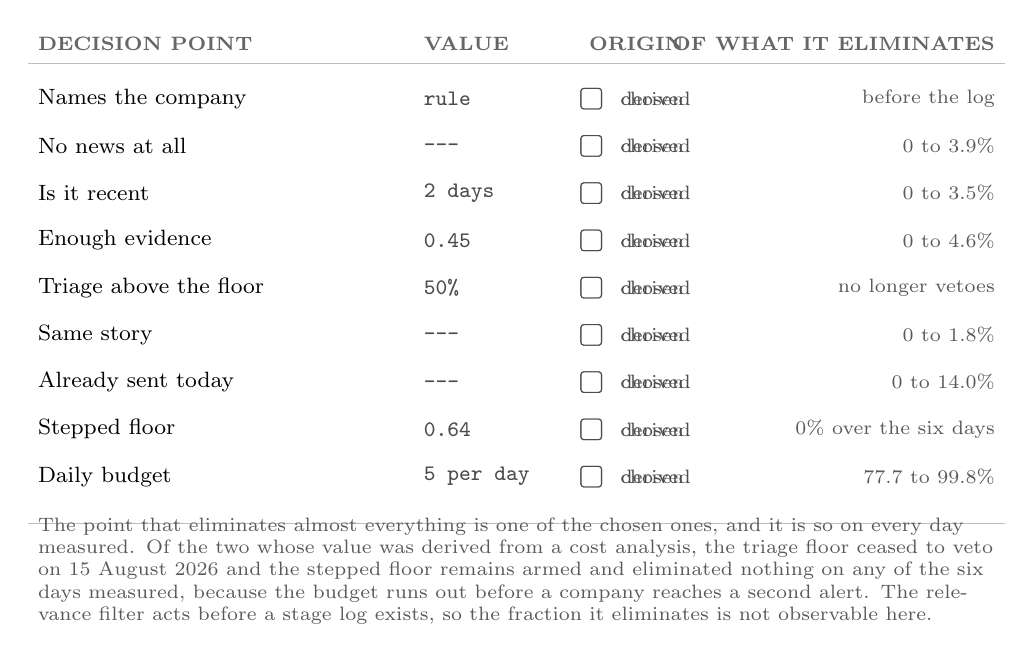
\begin{tikzpicture}[font=\footnotesize,
  lin/.style={align=left, anchor=west},
  val/.style={font=\footnotesize\ttfamily, anchor=west, text=black!70},
  der/.style={draw=black!70, fill=black!70, rounded corners=1pt},
  esc/.style={draw=black!70, fill=white, rounded corners=1pt},
  cor/.style={font=\scriptsize, anchor=east, text=black!65},
]
  % Cabecalhos
  \node[lin, font=\scriptsize\bfseries, text=black!60] at (0,0.75) {DECISION POINT};
  \node[val, font=\scriptsize\bfseries, text=black!60] at (4.9,0.75) {VALUE};
  \node[lin, font=\scriptsize\bfseries, text=black!60] at (7.0,0.75) {ORIGIN};
  \node[cor, font=\scriptsize\bfseries, text=black!60] at (12.4,0.75) {OF WHAT IT ELIMINATES};
  \draw[black!25] (0,0.5) -- (12.4,0.5);

  % (nome, valor, derivado?, quota, y)
  \foreach \nome/\valor/\tipo/\quota/\y in {
      {Names the company}/{rule}/{e}/{before the log}/{0.05},
      {No news at all}/{---}/{e}/{0 to 3.9\%}/{-0.55},
      {Is it recent}/{2 days}/{e}/{0 to 3.5\%}/{-1.15},
      {Enough evidence}/{0.45}/{e}/{0 to 4.6\%}/{-1.75},
      {Triage above the floor}/{50\%}/{d}/{no longer vetoes}/{-2.35},
      {Same story}/{---}/{e}/{0 to 1.8\%}/{-2.95},
      {Already sent today}/{---}/{e}/{0 to 14.0\%}/{-3.55},
      {Stepped floor}/{0.64}/{d}/{0\% over the six days}/{-4.15},
      {Daily budget}/{5 per day}/{e}/{77.7 to 99.8\%}/{-4.75}} {
    \node[lin] at (0,\y) {\nome};
    \node[val] at (4.9,\y) {\valor};
    \ifthenelse{\equal{\tipo}{d}}
      {\node[der, minimum width=2.6mm, minimum height=2.6mm, inner sep=0] at (7.15,\y) {};
       \node[lin, font=\scriptsize, text=black!70] at (7.4,\y) {derived};}
      {\node[esc, minimum width=2.6mm, minimum height=2.6mm, inner sep=0] at (7.15,\y) {};
       \node[lin, font=\scriptsize, text=black!70] at (7.4,\y) {chosen};}
    \node[cor] at (12.4,\y) {\quota};
  }

  \draw[black!25] (0,-5.35) -- (12.4,-5.35);
  \node[lin, font=\scriptsize, text=black!65, text width=12.2cm] at (0,-5.95)
    {The point that eliminates almost everything is one of the chosen ones, and it is so on every
     day measured. Of the two whose value was derived from a cost analysis, the triage floor ceased
     to veto on 15 August 2026 and the stepped floor remains armed and eliminated nothing on any
     of the six days measured, because the
     budget runs out before a company reaches a second alert. The relevance filter acts before a
     stage log exists, so the fraction it eliminates is not observable here.};
\end{tikzpicture}
\caption[The nine decision points, the origin of their value and what each one eliminates]{Each
decision point, the origin of the value it uses and the fraction of assessments that ends there,
measured over the production decision log across six days, between 19 and 21 August and between 3
and 5 September 2026. The column presents the range across those days and not a single value, since
the log keeps only three days at a time and the fractions vary with the day. The unit is the
assessment and not the news item: the system re-scores the same headlines at every sixty-second
cycle, so these values measure where the system's time is spent and not how many distinct stories
each point eliminated. The distinction between a derived value and a chosen value is the same as in
Table~\ref{tab:sis_portas}. The nine include the five shown in
Figure~\ref{fig:sis_caminho} plus four that act outside it: the absence of news, the
suppression of repeated stories, the stepped floor and the daily budget. The reading the
figure allows, and that the table alone does not give, is that the reduction in volume is not
made by the points whose value was derived: it is made by
the budget, whose value was chosen, and so it is on each of the six days. The values come from the
decision log published with the system.}
\label{fig:sis_razoes}
\end{figure}


\section{Construction of the explanation}
\label{sec:sis_explicacao}

The message delivered is not a single sentence, but a structure with four parts, always present
and always in the same order:

\begin{enumerate}
  \item the observed fact, expressed in values, with the source indicated;
  \item the past cases retrieved, presented individually, with date, similarity and subsequent
        movement;
  \item the caveat that the cases presented are observed history and not a forecast;
  \item the estimated probability of a market reaction, with no indication of direction.
\end{enumerate}

The order responds to two constraints. The fact precedes the statistic because an alert that opens
with a $z$ value loses the reader on the first line, and the recipient defined in
Chapter~\ref{cap:introducao} does not have the training that would make that value immediately
interpretable. The estimate occupies the last position because it is the only quantity in the
message that refers to the future, which ensures that a reading interrupted before the end retains
facts and history.

On the path started by a price movement, the first part also carries the statistical
characterisation in plain language, since in that case the observed fact is the movement itself. On
the path started by a news item, that position is occupied by the headline and the link to the
article.

The number of precedents presented is likewise a design decision. The system displays three of the
cases retrieved and not all of them, and the reason is not available space. Research on explanation
establishes that people look for selective and contrastive reasons, and not exhaustive enumerations
of the factors that contributed to an outcome \autocite{miller2019explanation}. A list of thirty
cases would be more complete and less usable. The same principle determines that the message
displays the quantities that support the decision and not the full computation that produced
them.

Figure~\ref{fig:sis_alerta} reproduces an alert exactly as it was delivered, copied from the
channel log without editing. The headline it quotes is reproduced verbatim, since translating or
paraphrasing quoted material would break the verifiability that the system exists to preserve.
% ⚠️ Na arvore PT segue-se aqui um paragrafo que justifica a mensagem estar em ingles enquanto
% a prosa esta em portugues. Nao se aplica nesta arvore, onde as duas estao na mesma lingua, e
% explica-lo descreveria uma divergencia que nao existe.

\begin{figure}[ht]
\centering
\begin{tcolorbox}[colback=black!3, colframe=black!35, boxrule=0.4pt, arc=2pt,
                  width=0.97\textwidth, fontupper=\ttfamily\scriptsize]
\textcolor{black!55}{[1]} News alert for AMZN (Amazon) (2026-08-13)\\
\hspace*{1em}"Prediction: Amazon Will Join Apple in the \$4 Trillion Club Before 2030"\\[4pt]
\textcolor{black!55}{[2]} 3 similar past headlines. Their 5-day move ranged -2.73\% to -2.73\%\\
\hspace*{1em}(average -2.73\%):\\
\hspace*{1em}-2.73\% in 5d · AAPL 2026-08-05 (8d ago) · "If You Invested \$100 In Apple\\
\hspace*{2em}Stock 10 Years Ago, You Would Have This Much Today" (sim 0.56)\\
\hspace*{1em}-2.73\% in 5d · AAPL 2026-08-05 (8d ago) · "Apple's Selloff Is Overdone"\\
\hspace*{2em}(sim 0.51)\\
\hspace*{1em}-2.73\% in 5d · AAPL 2026-08-05 (8d ago) · "Apple's Buyback Is Retiring\\
\hspace*{2em}Less Stock Just As The Memory Bill Grows" (sim 0.47)\\[4pt]
\textcolor{black!55}{[3]} 3 of 3 shown cases moved down — topic-similar past cases, not a\\
\hspace*{1em}prediction for this news (an observed pattern, not a forecast).\\
\hspace*{1em}Observed past outcomes after similar news, not a price prediction and\\
\hspace*{1em}not advice.\\[4pt]
\textcolor{black!55}{[4]} Materiality estimate (learned triage): 57\% chance of an unusually\\
\hspace*{1em}large move over the next few days, in EITHER direction — raised by\\
\hspace*{1em}recent volatility (20d) and sector; lowered by today's own move and\\
\hspace*{1em}recent momentum (5d). This estimates whether the market reacts, never\\
\hspace*{1em}which way: it is not a price forecast and not advice.
\end{tcolorbox}
\caption[Alert delivered to the channel]{Alert delivered on 13 August 2026, reproduced from the log
reproduced from the channel log, with typographic markers suppressed and the numbering of the four
parts added; no number, word or punctuation mark was altered. The numbers in square brackets
identify the four parts of the structure. Every
value comes from the component that computed it: the similarity, from the retrieval engine; the
five-day movement, from the impact measurement; and the probability of $57\%$, from the calibrated
model. Part \textnormal{[1]} contains a headline that is itself a forecast, with a target and a
horizon; it is third-party content reproduced literally, and Section~\ref{sec:met_etica} discusses
the reach of the no-forecast guarantee in that context. Part \textnormal{[2]} displays the
similarity as a raw value, faithful to what the engine computed and not interpretable by whoever
reads it.}
\label{fig:sis_alerta}
\end{figure}

The probability presented on the last line is not the raw score of the model. It results from its
conversion into a probability, by fitting a sigmoid over a held-out validation block
\autocite{niculescu2005calibration}. The distinction is operationally relevant: a raw score orders
the candidates without admitting interpretation in isolation, whereas a calibrated probability
establishes that, among the headlines to which the system assigns $57\%$, approximately that
fraction does show an unusual movement. It is the difference between a quantity usable only
internally and a quantity that can be presented.

The guarantee has declared limits. Section~\ref{sec:av_qi3} reports the mean error of this
probability and records that the calibration is fitted on a block whose prevalence does not
coincide with that of the block to which it is applied, which shifts the scale by about five
percentage points in the optimistic direction. The ordering between candidates is not affected,
since the transformation preserves the order; the absolute value announced is.

The last line of the alert does not merely present the probability: it names the inputs that
raise it and those that lower it. That enumeration is not drafted, it is read off the calculation
itself. Listing~\ref{lst:contrib} shows the operation that produces it. In a logistic regression
with standardisation, the logit is the sum of the constant term with the product of each
coefficient by the standardised value of the corresponding input, so each term of that sum is the
exact contribution of one input, and not an approximation obtained over the model after training.
The hundreds of dimensions of the headline vector are summed into a single term, so that the
message remains legible; the context inputs appear one by one. It is from this ordering that the
words \emph{``raised by recent volatility (20d) and sector; lowered by today's own move''} of
Figure~\ref{fig:sis_alerta} come.

\begin{lstlisting}[caption={[The additive decomposition the message states]The decomposition that
the last line of the alert states. The product of the coefficient vector by the standardised
vector gives the contribution of each input to the logit; the terms are grouped and ordered by
decreasing magnitude. The explanation presented to the user is this sum, and not a second model
fitted over the first. The internal documentation of the function is omitted.},
label={lst:contrib}]
scaler = pipeline.named_steps["scale"]
lr = pipeline.named_steps["lr"]
x_scaled = scaler.transform(np.asarray(x_row, dtype="float64").reshape(1, -1))[0]
contribs = lr.coef_[0] * x_scaled

grouped: dict[str, float] = {}
for name, c in zip(feature_names, contribs, strict=True):
    if name.startswith("emb_"):
        key = "headline content"
    elif name.startswith("sector_"):
        key = "sector"
    else:
        key = _FRIENDLY.get(name, name)
    grouped[key] = grouped.get(key, 0.0) + float(c)
return sorted(grouped.items(), key=lambda kv: -abs(kv[1]))
\end{lstlisting}

\subsection{Disagreement between the claim and the evidence}

The alert of Figure~\ref{fig:sis_alerta} presents three precedents with an identical impact of
$-2.73\%$, and an identical date. The coincidence is not accidental: the impact is measured per
pair formed by company and day, so three headlines of the same company on the same day share the
same value by construction. The wording \emph{``3 of 3 shown cases moved down''} presents as
agreement between three cases what is one day observed three times.

The extent of the problem was measured over the $247$ news alerts with precedents delivered
between 11 July and 13 August 2026. In $36.8\%$ of them the cases displayed rest on a number of
distinct days lower than the number of cases presented, and in $11.3\%$ the three cases correspond
to the same day. Of the $120$ alerts that claim unanimity of direction, $23.3\%$ rest on a single
day.

The effect is circumscribed. No metric reported in Chapter~\ref{cap:avaliacao} is affected, since
precision at $k$ counts headlines and direction agreement is measured pair by pair over the
historical corpus. What is affected is the strength the alert claims before the user, and
Chapter~\ref{cap:conclusoes} records the fact as a limitation.

\subsection{Web application}

The same information is made available in a web application, which allows what was delivered and,
above all, what was not, to be consulted. It is in that application that the decision log described
in Section~\ref{sec:sis_politica} resides. The design of the interface is not a contribution of
this dissertation and is therefore not described; presenting it is justified by its being the only
place in which the system's absence of communication is observable. Figures~\ref{fig:sis_pagina}, \ref{fig:sis_empresa} and~\ref{fig:sis_silencio} present, in that
order, the state of the day, the evidence for one company, and the record of a decision not to
communicate.

\begin{figure}[!htbp]
\centering
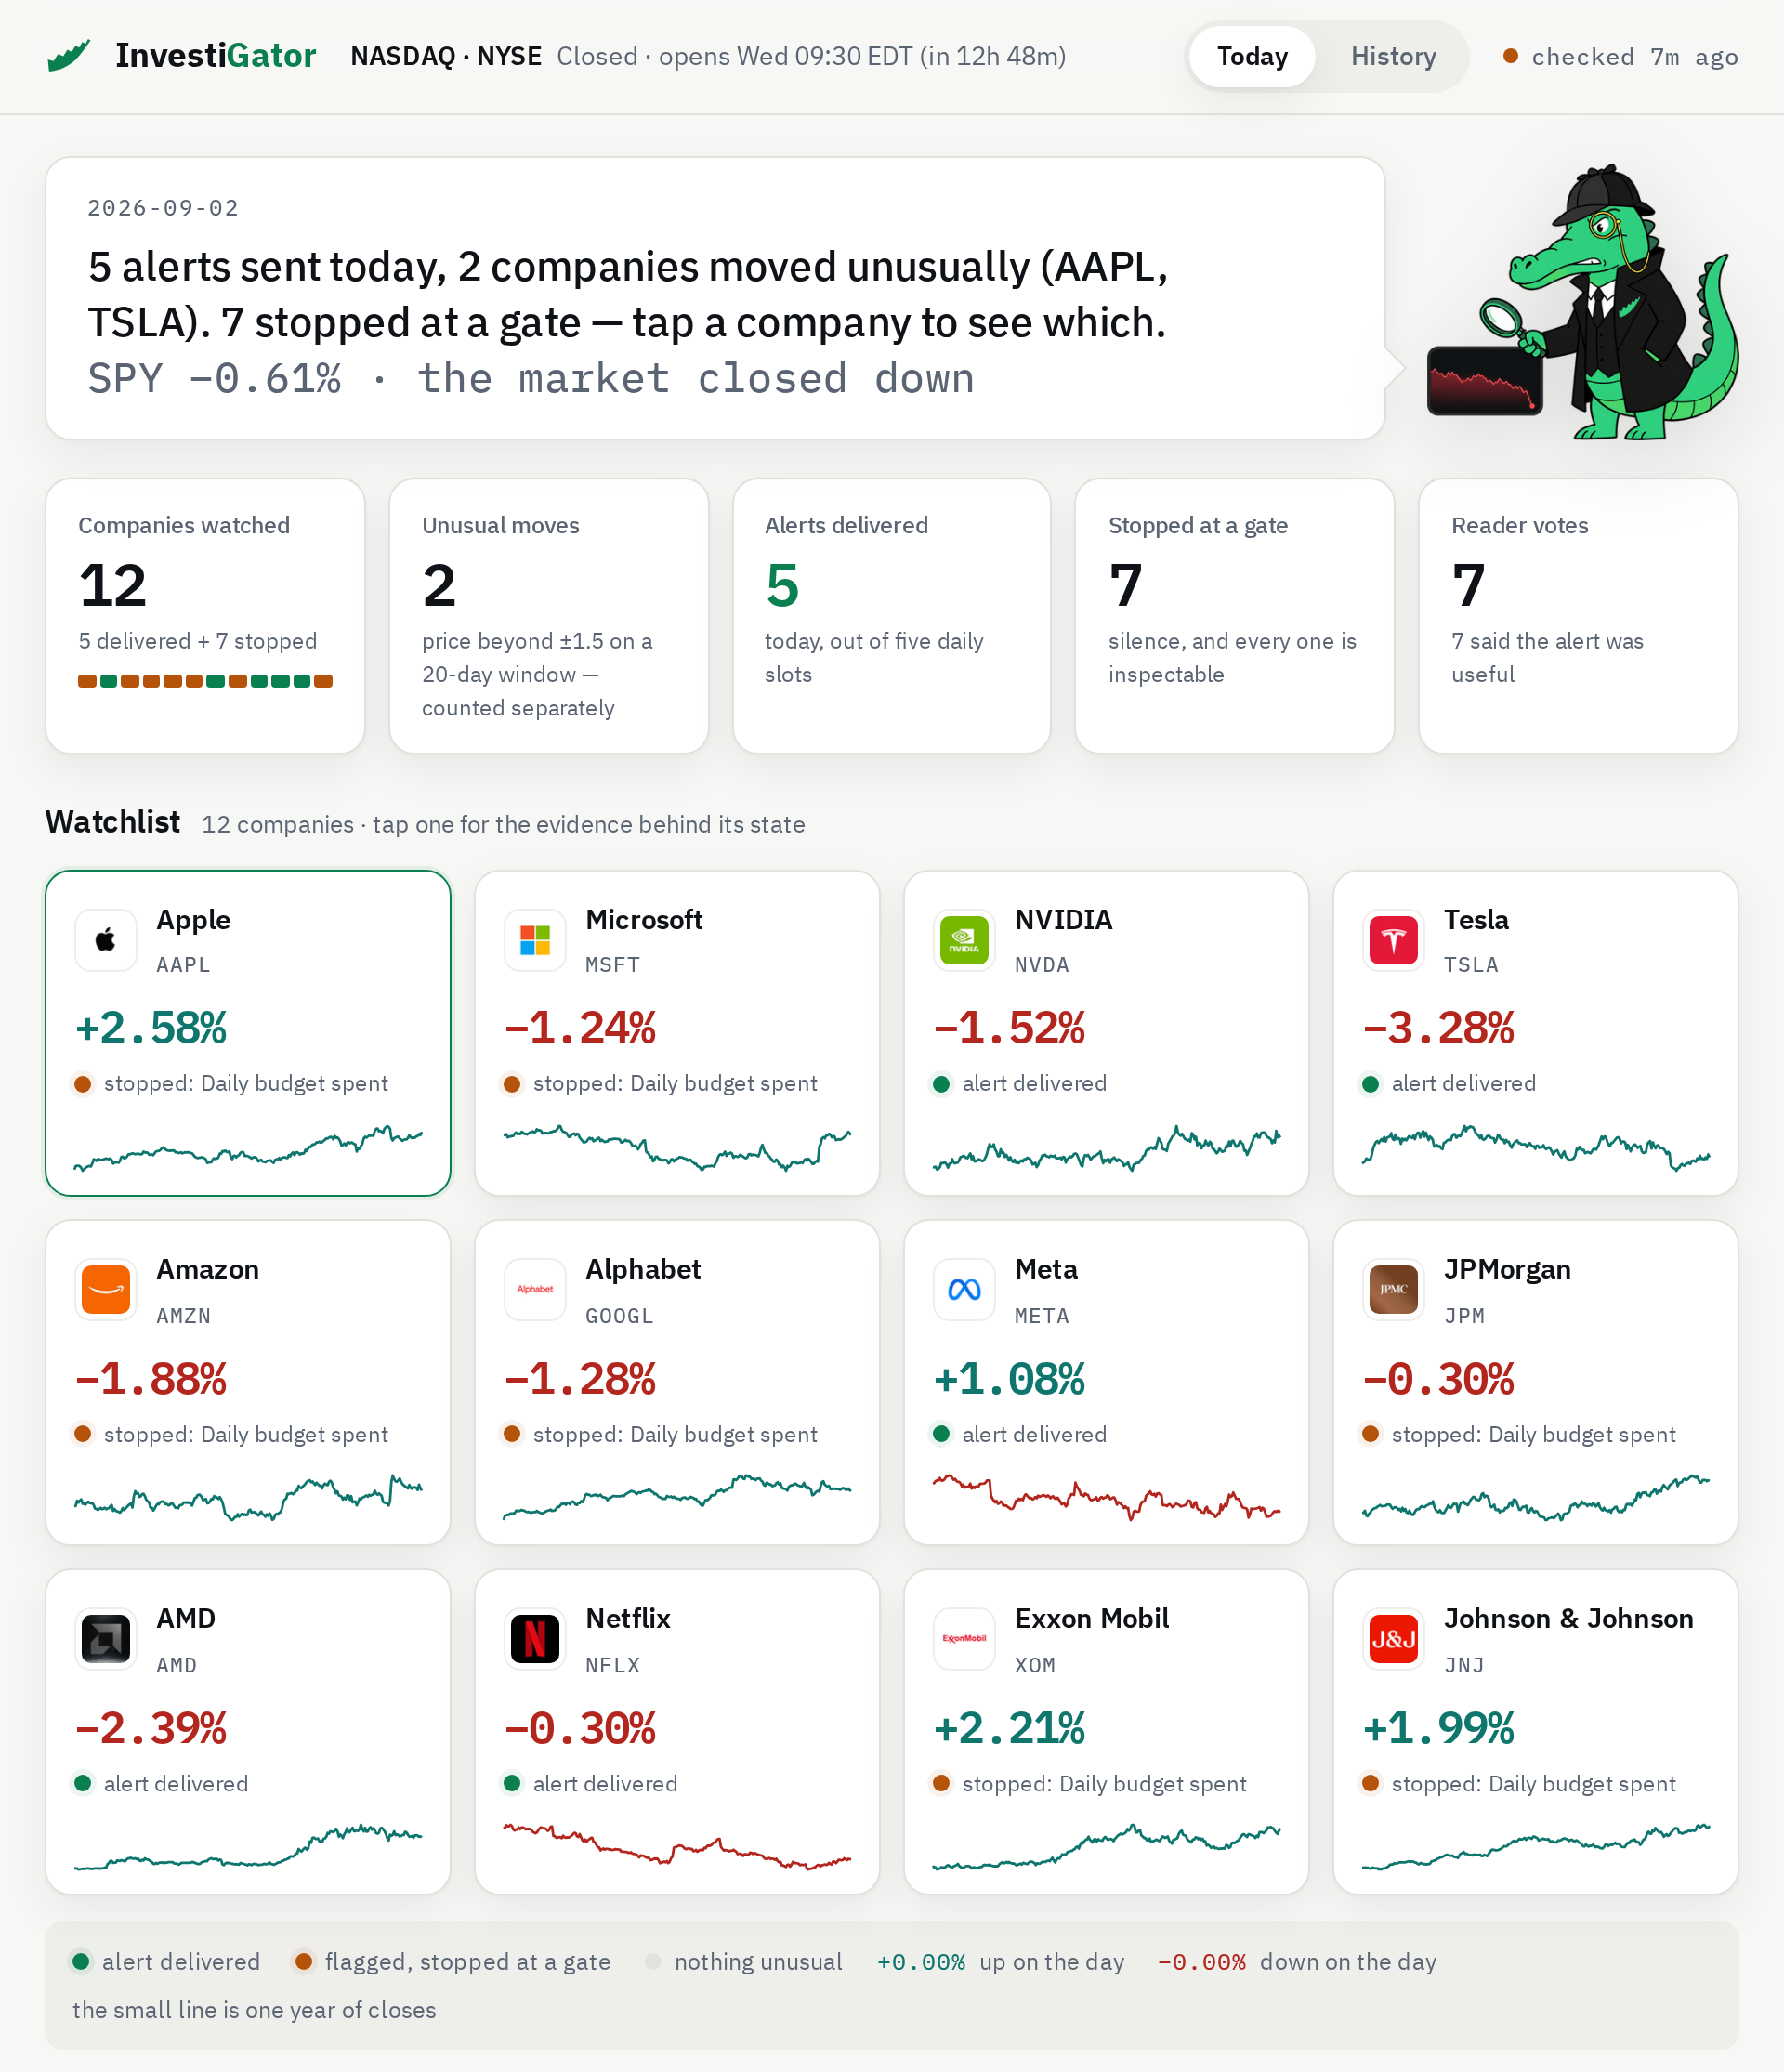
\includegraphics[width=0.95\textwidth]{figures/app_v7_painel.png}
\caption[State of the day in the web application]{Web application on 2 September 2026, with the
United States session closed. The five indicators split the twelve watched companies into five
alerts delivered and seven decisions not to communicate; the count of out-of-the-ordinary movements
measures something else, the price, and is therefore presented as a separate count. Each company
declares its state on the surface, and every colour used has a legend, including that of the
mascot, which follows the daily change of the market index used in the decomposition. The captures
are generated from a snapshot of the application itself, and not collected by hand; the capture
width is $960$ pixels, since that is the width at which the interface text stays legible after
being reduced to the text box of this document.}
\label{fig:sis_pagina}
\end{figure}

\begin{figure}[!htbp]
\centering
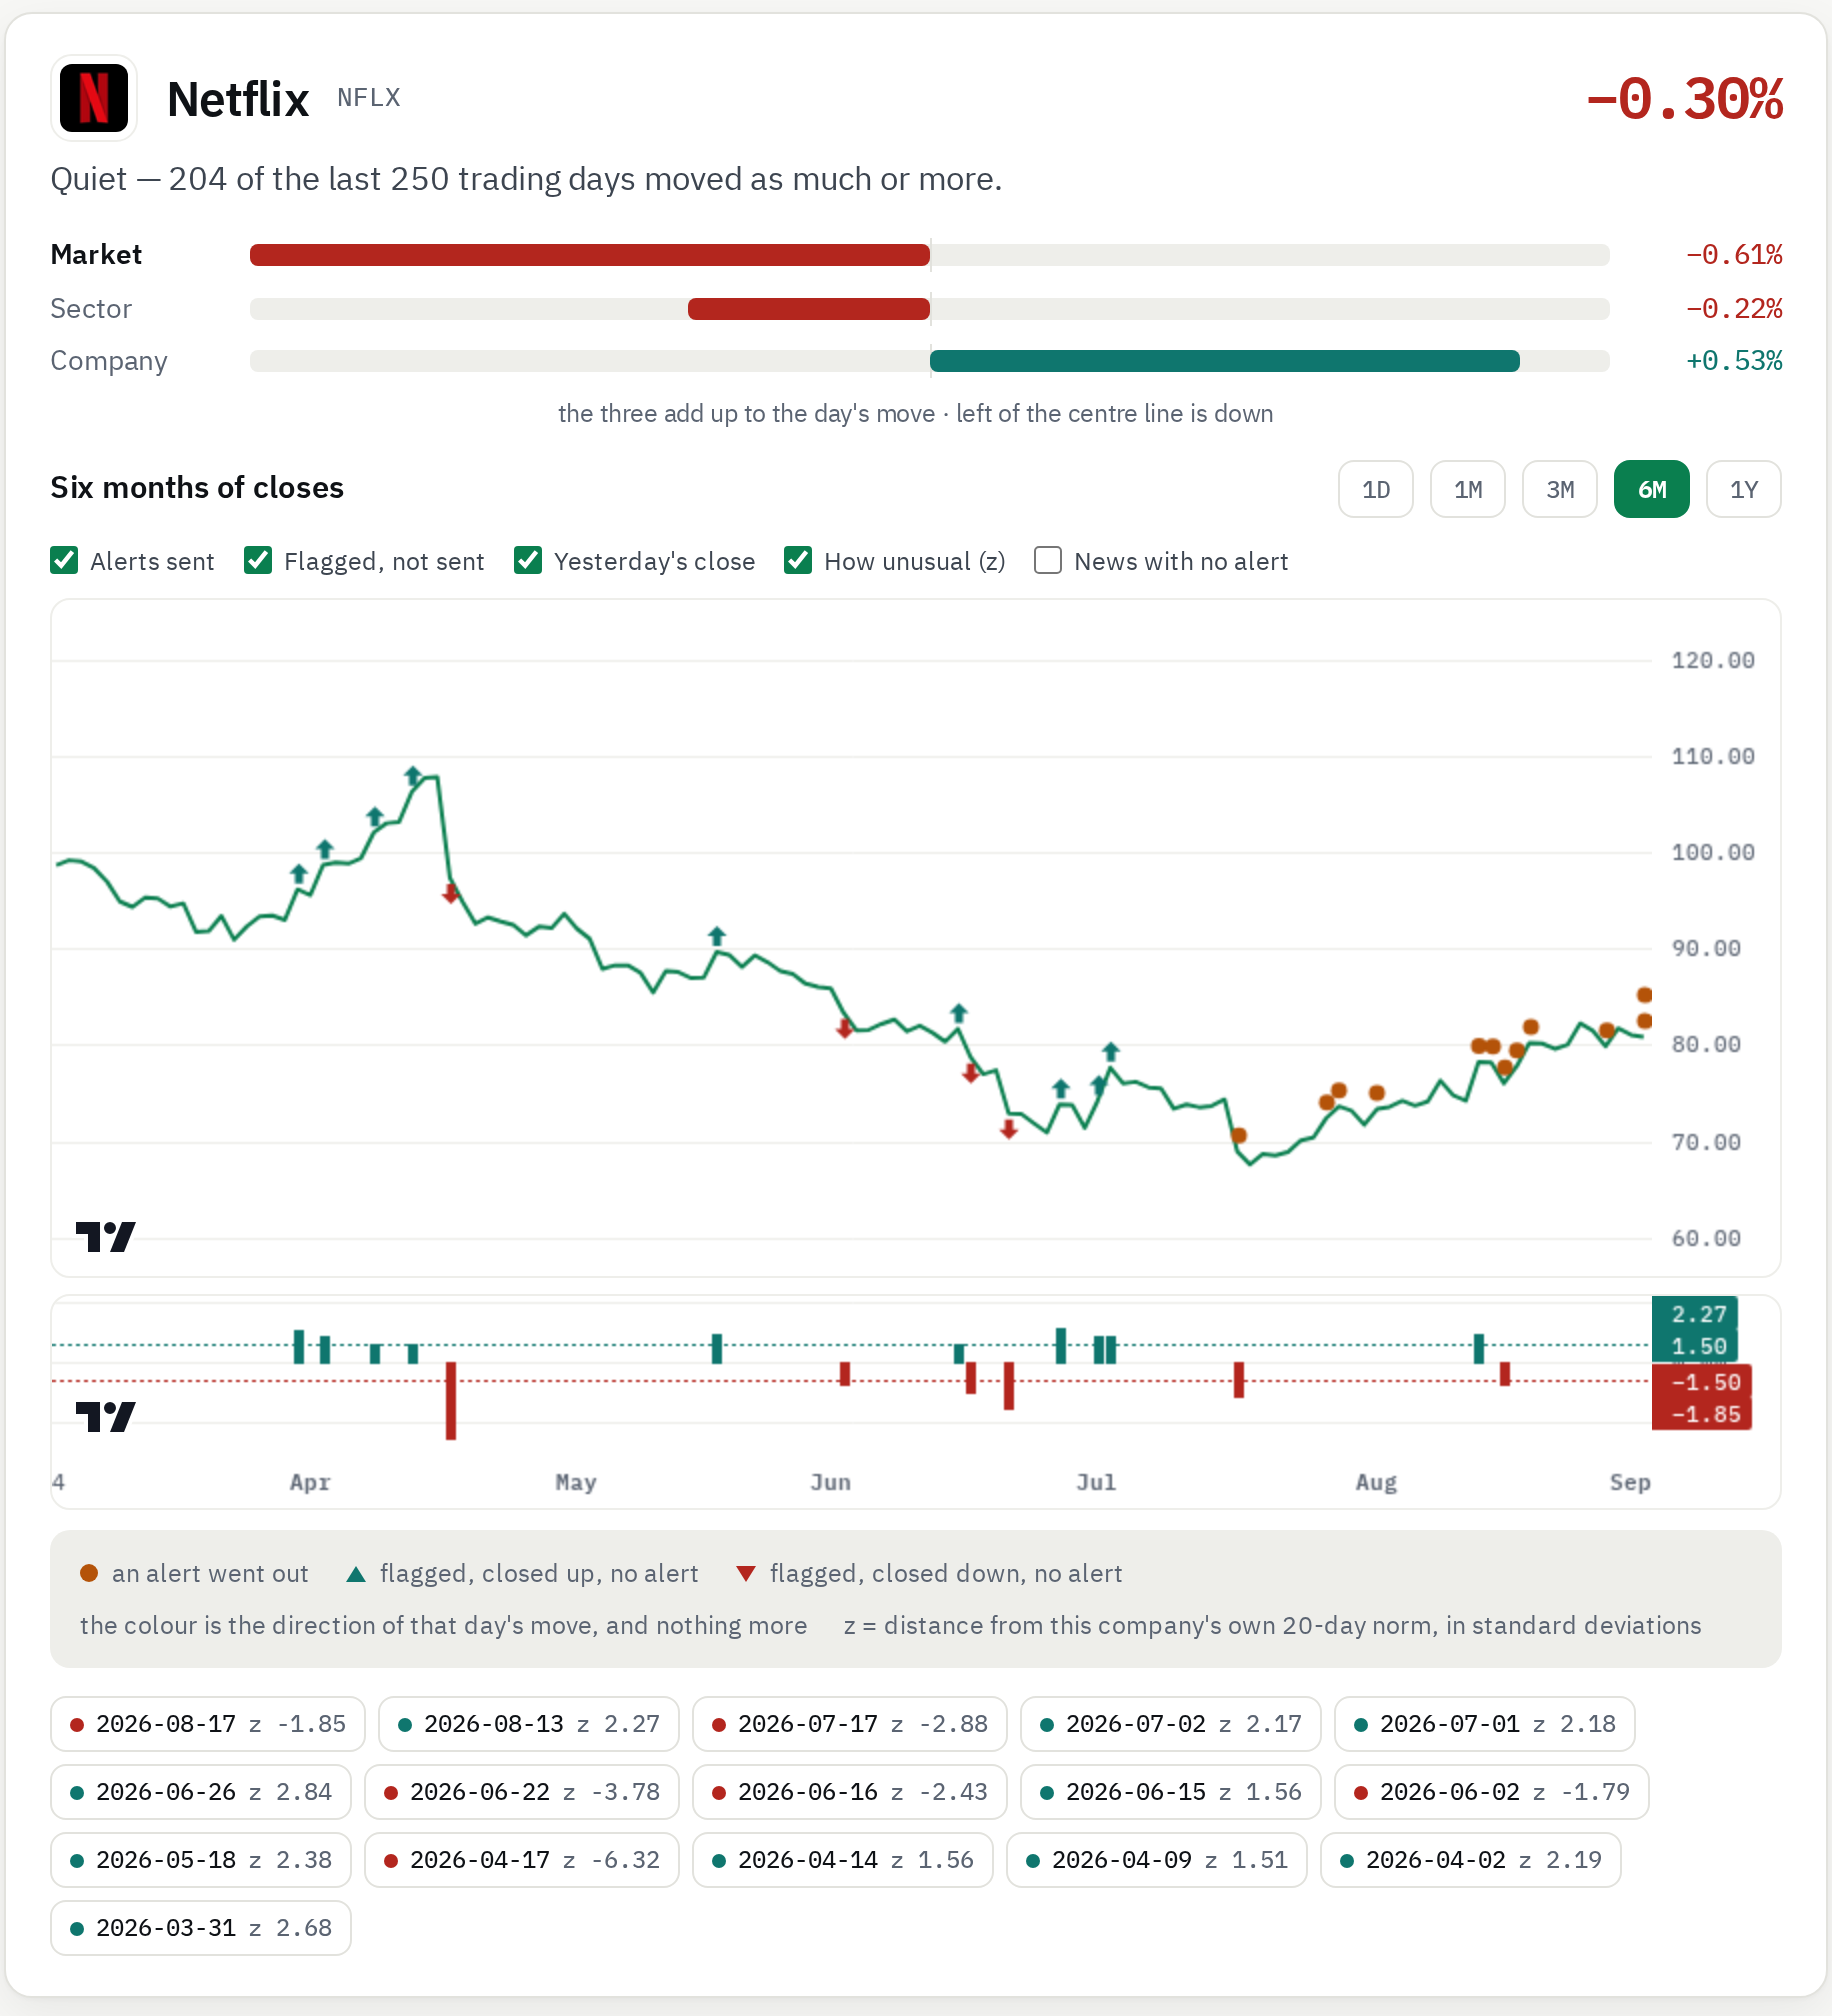
\includegraphics[width=0.94\textwidth]{figures/app_v7_empresa.png}
\caption[Evidence for one company]{View of one company: the verdict in words before any number,
the split of the movement into the three parts, and the price series. The marks separate the two
things this work distinguishes: the dot marks a day on which an alert was delivered, and the arrow
a day the detector flagged that no message accompanied. The lower band shows the $z$ value of those
days against the $\pm1.5$ threshold, on an axis of its own since it shares no unit with the price.
The direction of the arrow is that of the close and nothing more; the date and the $z$ value of
each day are on the cards below, and not on the line, so that they do not overlap. The interface
opens on the current day; the figure shows the six-month range, since that is the one in which the
distinction between flagging and communicating becomes observable.}
\label{fig:sis_empresa}
\end{figure}

\begin{figure}[!htbp]
\centering
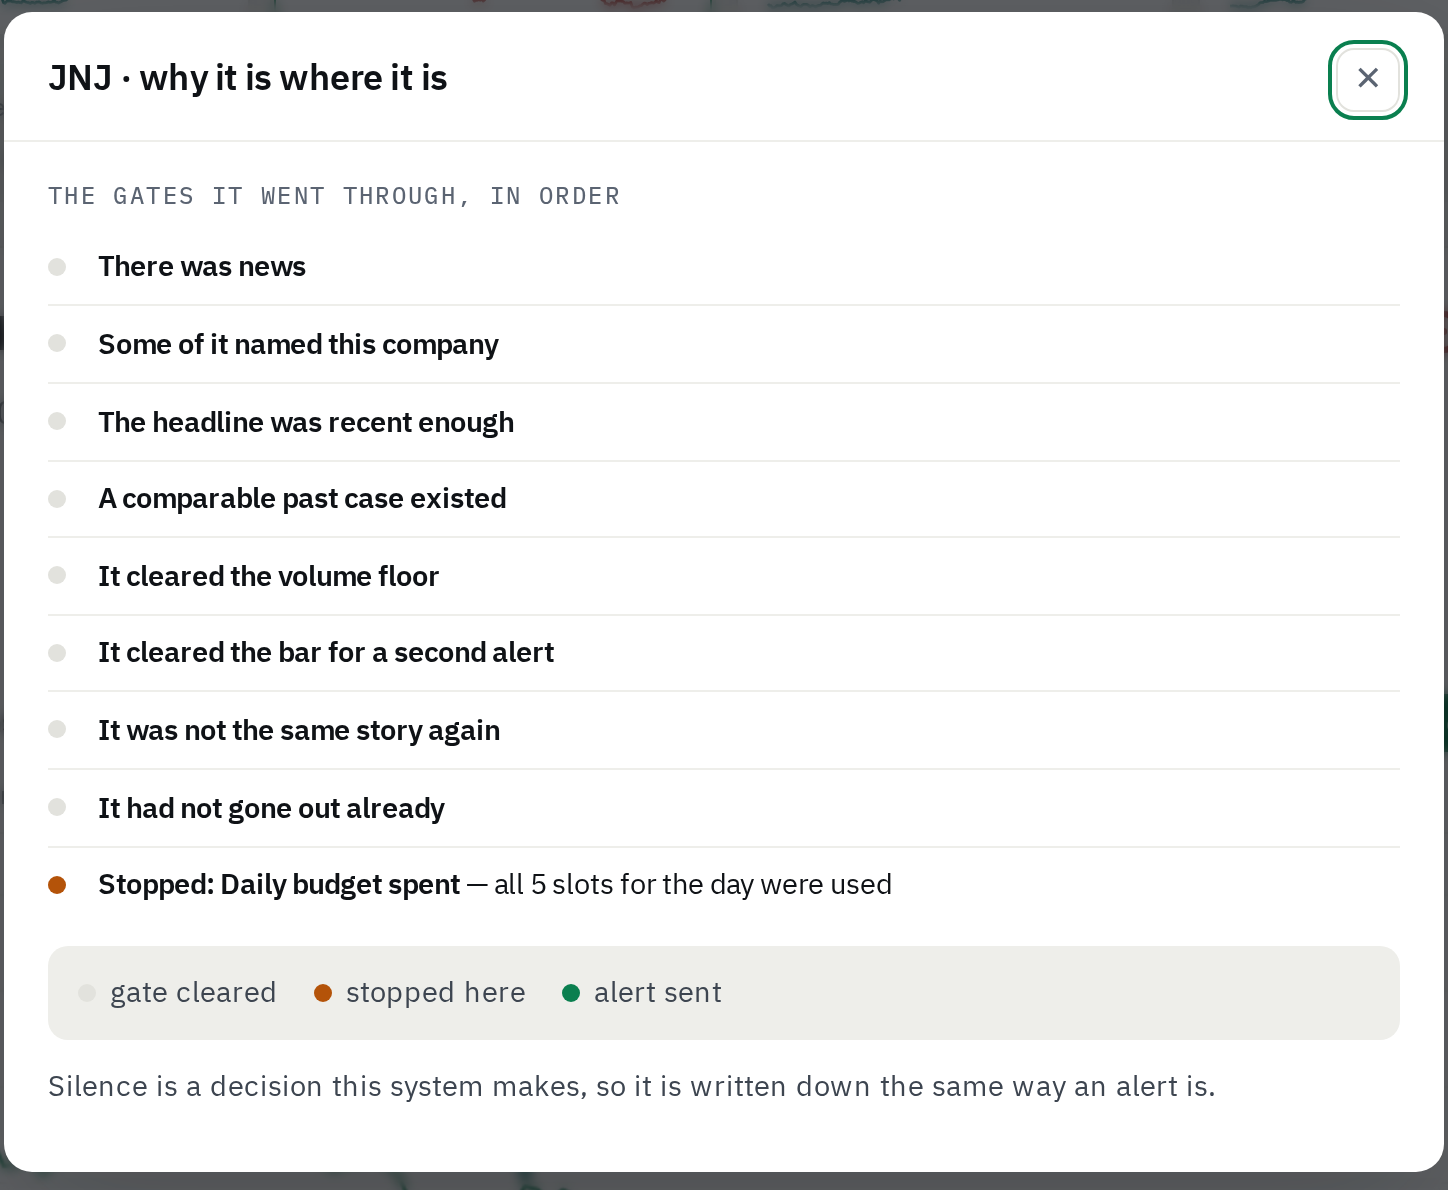
\includegraphics[width=0.72\textwidth]{figures/app_v7_silencio.png}
\caption[Record of a decision not to communicate]{The gates a company crossed, in the order of the
policy of Section~\ref{sec:sis_politica}. The gates crossed are stated by what the company
satisfied; only the one at which it stopped is stated by the rejection, with the concrete reason.
Silence is here a recorded decision, and not an absence of information.}
\label{fig:sis_silencio}
\end{figure}

The company of Figure~\ref{fig:sis_empresa} is an illustrative case of the investor's second
question, through the disagreement between the percentage change and the split. The stock recorded
a fall of $0.30\%$, and the company-specific part was $+0.53\%$ — positive. The fall came from the
market, at $-0.61\%$, and from the sector, at $-0.22\%$. The percentage change alone indicates that
the company fell and leads to the search for an internal cause that does not exist; the split shows
that the company rose against a falling market. The verdict classifies the day as ordinary: $204$
of the last $250$ trading days recorded an equal or larger change.

Figure~\ref{fig:sis_silencio} shows the same requirement on the side of silence. On that day, the
seven companies that generated no alert all stopped at the same gate: the daily budget of five
alerts, exhausted at $14$:$02$~UTC. The important reading is not the number, but the form: the
company crossed eight gates, each stated by the criterion it satisfied, and stopped at a design
constraint declared from the outset. None of the gates crossed is presented as a failure, which
avoids the inverse reading that the previous version of the interface allowed.

\section{Deployment and operation}
\label{sec:sis_operacao}

The system runs as a permanent process, with a sixty-second scan cycle, on hosting credits
included in an academic plan. The first version used a free best-effort scheduler, whose effective
period was approximately one and a half hours. The change to a permanent process was motivated by
reducing the delay of the alerts.

Latency was measured over the $278$ news alerts delivered between 29 July and 30 August 2026 that
record a publication time and a send time. The median of the complete path is $353$ minutes, with a
ninetieth percentile of $964$ minutes. The breakdown locates that time without ambiguity: the
median between publication and detection is $353$ minutes, and the median between detection and the
arrival of the message is $5$ seconds, with a ninetieth percentile of $16$ seconds. The system
delivers in seconds what the source gives it.

The separation by configuration does not confirm the expectation that motivated the change. Over
the $28$ alerts delivered by the scheduler the median is $196$ minutes; over the $250$ delivered by
the permanent process it is $402$ minutes. The shorter cycle did not reduce the observed latency.
The comparison is not interpretable as an effect of the cycle, since the two configurations did not
operate in parallel, the news sources and the calendar period changed between them, and the samples
are of very unequal size. What the measurement establishes is that shortening the cycle would only
pay off if the time were in the cadence with which the system consults the source, and it is
not.

Three causes contribute to the delay in discovery, and this history does not separate them. The
first is the source listing the news hours after the time it itself declares. The second is that
the most recent item in the feed is not the most recent \emph{relevant} one: in a sample collected
on 7 August 2026, the feed of one of the companies carried $250$ headlines with the most recent
published at 11:39, but the most recent among the $30$ relevant ones was from 08:14. The alert goes
out on the correct headline, and it is that headline that is old. The third is that the daily
budget is already spent, which does not appear in this measurement because an alert that is not
delivered records no send time. Only the first would be mitigated by a paid news service, and its
contribution is not measured.

All these values are a lower bound on the latency felt by the user, since the publication time is
the one declared by the source and not the instant of the event.

\subsection{Growth of the case base}
\label{sec:sis_base}

Every relevant headline observed by the scan is kept as a candidate precedent. Eight days later,
when the impact on the price becomes observable, the candidate is measured by the same alignment
rule of Section~\ref{sec:met_recuperacao} and joins the case base. The waiting interval is not
inefficiency: it is the condition that prevents a case from knowing its own outcome.
Figure~\ref{fig:sis_ciclo_kb} represents the cycle.

\begin{figure}[ht]
\centering
\begin{tikzpicture}[font=\footnotesize, >={Stealth[length=2.2mm]},
  et/.style={draw, rounded corners=3pt, align=center, inner sep=4pt, text width=2.65cm,
             minimum height=1.25cm, fill=black!5},
  esp/.style={draw, dashed, rounded corners=3pt, align=center, inner sep=4pt, text width=2.4cm,
              minimum height=1.25cm, fill=white},
]
  \node[et]  (a) at (0,0)     {\textbf{day $t$}\\ the scan observes a relevant headline};
  \node[esp] (b) at (3.55,0)  {kept as a candidate, with its vector};
  \node[et]  (c) at (7.0,0)   {\textbf{day $t+8$}\\ the impact is observable};
  \node[et]  (d) at (10.5,0)  {joins the \textbf{case base}};

  \draw[->, thick, black!55] (a) -- (b);
  \draw[->, thick, black!55] (b) -- (c);
  \draw[->, thick, black!55] (c) -- (d);

  \draw[->, thick, black!55] (d.south) -- ++(0,-0.85) -| (a.south)
    node[pos=0.25, below, font=\scriptsize, black!65]
    {later evaluations compare against the cases already matured};
\end{tikzpicture}
\caption[Growth cycle of the case base]{Path of a headline between its observation and its
availability as a precedent. The eight-day interval follows from the impact of a case being
observable only after the price movement. The cycle keeps up to date the evidence the system
presents, and not the parameters of the model: no component is retrained.}
\label{fig:sis_ciclo_kb}
\end{figure}

The mechanism updates the evidence displayed and not the parameters of the model. In the concept
drift taxonomy of \textcite{gama2014survey}, the system has detection of the change and not
adaptation to it.

It was found, with the system already in operation, that this cycle had been interrupted for
nineteen days without any error being recorded. The two processes run on separate machines whose
file system is reinitialised at every start, and the intermediate maturation files were not being
published to the shared data store. It corresponds to the class of cost that
\textcite{sculley2015debt} call an undeclared data dependency: each component fulfils its contract,
and the assumption that links them is expressed nowhere. Chapter~\ref{cap:conclusoes} returns to
the case as a limitation.

\section{Life cycle of the learned component}
\label{sec:sis_ciclo}

The system trains a single model, the nine-input logistic regression described in
Section~\ref{sec:met_triagem}. Measured against a one-variable baseline, that model performs worse,
a result reported in Section~\ref{sec:av_qi3}.

The engineering contribution does not lie in the size of the model, but in the infrastructure that
makes that result, and the negative conclusion it supports, defensible. That infrastructure has
seven components, each of which exists because its absence would produce a favourable and
unverifiable result. Figure~\ref{fig:sis_lifecycle} represents the two halves of the cycle.

\begin{figure}[ht]
\centering
\begin{tikzpicture}[font=\scriptsize, >={Stealth[length=2mm]},
  cx/.style={draw, rounded corners=2pt, align=center, inner sep=3pt, text width=2.15cm,
             minimum height=1.0cm, fill=black!5},
  art/.style={cx, fill=black!14, draw=black!55, thick},
  obs/.style={cx, fill=white, draw=black!45},
  fase/.style={font=\scriptsize\bfseries, text=black!60},
]
  \node[fase] at (-1.55,0.95) {construction};
  \node[cx]  (d) at (0,0)    {labelled dataset};
  \node[cx]  (t) at (2.5,0)  {training};
  \node[cx]  (v) at (5.0,0)  {validation\\ \emph{calibration}};
  \node[cx]  (s) at (7.5,0)  {test\\ \emph{single use}};
  \node[art] (m) at (10.0,0) {versioned artefact};

  \foreach \xa/\xb in {d/t, t/v, v/s, s/m} \draw[->, thick, black!55] (\xa) -- (\xb);

  \node[fase, anchor=west] at (-1.1,-2.7) {observation};
  \node[art] (p) at (0,-1.9)   {the \textbf{same} model, in production};
  \node[obs] (g) at (2.5,-1.9) {log of every decision};
  \node[obs] (w) at (5.0,-1.9) {wait for the price to respond};
  \node[obs] (r) at (7.5,-1.9) {post-validation and drift};

  \draw[->, thick, black!55] (m.south) -- ++(0,-0.5) -| (p.north);
  \foreach \xa/\xb in {p/g, g/w, w/r} \draw[->, thick, black!55] (\xa) -- (\xb);

  \draw[->, dashed, black!40] (r.east) -- ++(0.9,0) |- (10.0,-1.05);
  \node[align=center, text width=1.3cm, text=black!70] at (10.4,-1.9)
    {retraining:\\ \textbf{absent}};
\end{tikzpicture}
\caption[Life cycle of the learned component]{The two halves of the cycle. In the upper half,
construction: the data are labelled, the split is chronological, the calibration is fitted on the
validation block and the test block is used only once. In the lower half, observation: the model in
production is the model evaluated, every decision is logged, and days later it is confronted with
the movement actually observed. The dashed link would close the cycle and does not exist: drift is
measured and is not corrected.}
\label{fig:sis_lifecycle}
\end{figure}

\begin{description}
  \item[Construction of the dataset.] \gls{FNSPID} supplies dated headlines, and the prices come
        from a distinct source. The alignment of the two series, the assignment of a Saturday news
        item to the corresponding trading day, and the derivation of the label from the future
        movement constitute the work that produces the $79{,}753$ examples of
        Section~\ref{sec:met_dados}.

  \item[Declaration of the label as a decision.] The existence of an abnormal movement in the
        following three days is not a fact present in the data: it is a definition, with a chosen
        threshold and horizon. Section~\ref{sec:av_qi3} measures nine alternative definitions
        instead of assuming the one adopted.

  \item[Verification of the temporal separation.] To the chronological blocks and the embargo is
        added an executable test, reproduced in Listing~\ref{lst:lookahead}: if the future of an
        example is perturbed, its inputs must stay unchanged and its label must change. The
        absence of leakage thus goes from a claim to a property verified at every run.

  \item[Calibration with measured bias.] The output of the classifier is a value in the unit
        interval, which serves both to rank candidates and to exclude them. The Platt fit runs on a
        block that never took part in training, and the prevalence discrepancy between that block
        and the test block is declared in Chapter~\ref{cap:avaliacao} instead of being left
        implicit.

  \item[Versioning of the artefacts.] The trained model, the calibrator and a descriptor of the
        run, containing the size of each block, the prevalence, the seed and the metrics, are kept
        with the dissertation. A metric unaccompanied by the artefact that produced it is not
        reproducible.

  \item[Identity between the model evaluated and the model deployed.] The sentence encoder used in
        the evaluation depends on a library whose size exceeds the production container. Instead of
        substituting another model, which would make the dissertation describe a system distinct
        from the one in operation, the same model was exported to a lightweight execution format
        and the fidelity of the conversion was measured.

  \item[Observation of the deployed system.] Every triage decision is logged. Once the necessary
        days have passed, a second procedure labels those decisions by the same rule used in
        training and measures the contribution of the model. It was by this route that the absence
        of contribution reported in Section~\ref{sec:av_qi3} was established. The drift of the
        inputs is measured by the same mechanism.
\end{description}

\subsection{Components developed and components consumed}

The only model consumed from outside is a pre-trained sentence encoder, used without any tuning.
The work claims no contribution over that component beyond its selection by measurement, carried
out against four alternatives, among them a larger model, two more recent encoders and a model
specific to the financial domain, which had the worst performance of the set. The dependency is
essential, since there is no semantic retrieval without sentence representation, and it is at the
same time replaceable: the interface that isolates it has an alternative implementation that
degrades to lexical overlap when the model is not available.

Everything else was developed within this work. The labelled dataset and the alignment procedure
that protects it from temporal leakage. The detector, with the estimation window that excludes the
day being explained. The split of the movement with shrinkage of the coefficients. The precedent
base with measured impact. The triage classifier and its calibration. The decision policy and the
constants of Table~\ref{tab:sis_portas}. The layer that composes the text from the computed
objects. And the mechanism that observes the system after deployment.

The system does not integrate a language model in the production of the text delivered to the
user. The absence is deliberate and follows from the argument developed in
Section~\ref{sec:ctx_xai}: a generated sentence is a statement, whereas the system described
delivers statements accompanied by the evidence that supports them.

A grounded generation layer is, even so, implemented and evaluated, and is not exposed. In it,
every sentence must cite a fact from the evidence bundle that accompanies it, and a check rejects
any sentence whose number does not belong to the fact it cites. Over a corpus of twenty-three
attempts to circumvent that check, all were rejected, and over eight faithful texts none was; in
the sections actually composed not a single delivered violation was recorded. The reason for not
exposing it is not the performance of that check, but the nature of the guarantee: in the text
delivered to the user the composition starts from a closed vocabulary, whereas the check of the
generated layer enumerates what it forbids, and an enumeration of the forbidden is weaker than an
enumeration of the permitted. No comparison with a complete retrieval-augmented generation
architecture was carried out, so nothing is asserted about what it would add.

\subsection{The missing link: retraining architecture}

The cycle does not include retraining. The parameters correspond to the period from 2018 to 2023
and were not readjusted, even though drift is measured and the population stability index places
the main input in the band of significant displacement. The operation would be technically
possible, since new labels derive from observed prices; the impediment is that retraining with the
production log would change the values reported in this document, and assessing that change
requires observation time which, at the date this chapter was written, did not exist.

The instrumentation that would make it possible was built and deployed on 4 September 2026, and
the log came to store, per decision, the value of each input, the date of the last price bar used
and the identity of the model. Two restrictions limit what can be drawn from it, and both were
fixed before any candidate existed. The first is that only decisions whose price bar is prior to or
equal to the date of the news are usable, since a later bar would describe a market that has
already observed the outcome the label measures. The second is that the unit of analysis is the
pair formed by company and day, and not the headline, which substantially reduces the number of
independent observations available in a short window. Nothing is asserted in this document about
the result of that comparison.

The absence of execution does not, however, dispense with defining the architecture.
Figure~\ref{fig:sis_retreino} presents the continuous training cycle designed for this system, with
the mechanisms that would make it safe. Three decisions characterise it.

The first is the \textbf{trigger}, conditional and not temporal. Retraining is set off when the
\gls{PSI} of any input exceeds $0.25$, the conventional threshold of significant
displacement, or after three months without review. The second is the \textbf{rolling window}:
training covers the twenty-four months preceding the trigger, and validation and test the following
periods, with the five-day embargo of Section~\ref{sec:met_triagem}. The split stays chronological,
because the problem does not cease to be temporal just because the model is new.

The third, and the one that distinguishes a continuous training cycle from dangerous automation,
is the \textbf{promotion gate}. A newly trained model does not replace the model in force by virtue
of being more recent: it replaces it only if it beats it over the same held-out test block, and if
the confidence interval of the difference excludes zero. A model that does not pass that gate is
logged and discarded, and the model in force remains with the drift declared. It is the difference
between adapting to change and chasing noise.

\begin{figure}[ht]
\centering
\begin{tikzpicture}[font=\scriptsize, >={Stealth[length=2mm]},
  cx/.style={draw, rounded corners=2pt, align=center, inner sep=3pt, text width=2.35cm,
             minimum height=0.95cm, fill=black!5},
  gat/.style={cx, dashed, fill=black!12},
  art/.style={cx, fill=black!16, draw=black!55, thick},
]
  \node[cx]  (p) at (0,0)     {decision log in production};
  \node[cx]  (m) at (2.9,0)   {maturation:\\ 8 days};
  \node[cx]  (r) at (5.8,0)   {new labels, from the same rule};
  \node[gat] (g) at (8.7,0)   {\textbf{trigger}\\ PSI $>0.25$\\ or 3 months};
  \node[cx]  (t) at (8.7,-1.9) {retraining over a 24-month window};
  \node[cx]  (v) at (5.8,-1.9) {fresh validation and calibration};
  \node[gat] (q) at (2.9,-1.9) {\textbf{promotion gate}\\ beats the one in force?};
  \node[art] (n) at (0,-1.9)   {promote\\ and version};

  \foreach \a/\b in {p/m, m/r, r/g} \draw[->, thick, black!55] (\a) -- (\b);
  \draw[->, thick, black!55] (g) -- (t);
  \foreach \a/\b in {t/v, v/q, q/n} \draw[->, thick, black!55] (\a) -- (\b);
  \draw[->, thick, black!55] (n.north) |- ++(0,0.75) -| (p.south);
  \draw[->, dashed, black!45] (q.south) -- ++(0,-0.55)
    node[below, align=center, black!60] {does not win:\\ log and discard};
\end{tikzpicture}
\caption[Retraining architecture designed and not executed]{Continuous training cycle defined for
this system and not executed within this work. The trigger is conditional and not temporal; the
window is rolling and the split stays chronological with embargo; and the promotion gate prevents a
new model from replacing the model in force without beating it over a held-out block. The dashed
link is the rejection path, and its existence is what distinguishes the cycle from automation that
chases noise.}
\label{fig:sis_retreino}
\end{figure}

The cycle likewise includes no form of human ground truth. The three labels used in this work,
corresponding to abnormal movement, membership of the same sector and percentile of movement, are
verifiable approximations that were never confronted with the judgement of a human assessor. It is
the limitation on which the others most depend, and Chapter~\ref{cap:conclusoes} returns to it.
